\documentclass{report}

\input{preamble}
\input{macros}
\input{letterfonts}

\title{\Huge{Software Engineering}\\Sem 2}
\author{\huge{Aditya Kumar}}
\date{}

\begin{document}

\maketitle
\newpage% or \cleardoublepage
% \pdfbookmark[<level>]{<title>}{<dest>}
\pdfbookmark[section]{\contentsname}{toc}
\tableofcontents
\pagebreak

\chapter{Introduction}
\section{Syllabus Overview}
Software engineering is the disciplined, step-by-step process of taking a software idea from conception all the way to a maintained, quality product — and this notes covers every major phase of that journey.

\begin{eli5}
	Imagine you and your friends want to build the coolest treehouse ever. You can't just grab wood and nails and hope for the best. First you talk about what you want (requirements). Then you draw a plan (design). Then you actually build it (coding). Then you check if it's safe and fun (testing). Then you fix stuff when a plank breaks later (maintenance). And you make sure it's sturdy enough to last (quality). Software engineering is learning all those steps properly — so your treehouse doesn't fall down on day one.
\end{eli5}

\img{1.png}

Engineering, in any discipline, means applying proven principles to build something reliably and systematically. Mechanical engineering does this for machines. Civil engineering does this for structures. Software engineering does this for software — taking an idea from someone's head and turning it into a working, maintainable product through a defined process.\\This syllabus is ~80–85\% theoretical, with a small numerical portion. The theoretical weight does not mean it is unimportant — in fact, software engineering concepts directly govern how every real software company operates. The lectures approach all theory through real-life examples to stop it from feeling abstract.\\Here is everything the syllabus covers, in order:
\begin{enumerate}
    \item \textbf{Introduction} - What software engineering is, why it exists, its advantages and disadvantages, basic applications, and the difference between a 'software' and a 'project'. The core idea: just as mechanical engineering gives you the principles to design machines, software engineering gives you the principles to design software systems.
    \item \textbf{Software Development Life Cycle (SDLC) — most important topic} - DLC is the step-by-step recipe for building software. It tells you what to do first, second, third — so that the final product matches what the client wanted, on time and within budget. The specific phases inside SDLC are covered individually below (requirement, design, implementation, testing, maintenance). SDLC questions are guaranteed in both competitive and university exams.

    \item \textbf{DLC Models — conventional and modern} - These are specific ways of executing the SDLC phases. Conventional models include the Waterfall model (strict, linear, one phase must finish before the next begins). Modern/iterative models include the Incremental model, Prototype model, and Spiral model. Each model is a different philosophy about how to handle uncertainty and change during software development.

    \item \textbf{Requirement Analysis} - Before building anything, you must gather exactly what needs to be built. This phase produces the SRS — Software Requirements Specification — a formal document that acts as a contract between the client and the development team. It captures functional and non-functional requirements with enough detail that no ambiguity remains. SRS preparation is asked in placements too.

    \item \textbf{Software Project Management} - Once requirements are clear, you must plan the project: how long will it take, how much will it cost, what can go wrong. This phase covers cost estimation (using metrics like Lines of Code and Function Points), time estimation, and risk analysis. The COCOMO model is the key numerical topic here and is heavily asked in competitive and university exams. The analogy: before building a house, you estimate material costs, labour time, and risks like floods or earthquakes in that area not after.

    \item \textbf{Software Design} - Before coding begins, a blueprint must be created. Software designers produce DFDs (Data Flow Diagrams), UML diagrams, and class diagrams that specify how the system will be structured. The two most exam-important design concepts are coupling (how much modules depend on each other — lower is better) and cohesion (how focused each module is on one job — higher is better). These are also directly used when writing project reports and research reports.
    \item \textbf{Implementation (Coding)} - The actual construction phase — translating the design into working code. Software engineering does not teach you to code here; it tells you that this phase comes after design is locked, and governs how it fits into the larger process.

    \item \textbf{Testing (2nd most important topic)} - After implementation, the software must be verified. Testing types covered include: unit testing (individual components), integration testing (components working together), system testing (the full system), white-box testing (testing internal logic — you can see the code), and black-box testing (testing external behaviour — you cannot see the code). Testing questions are guaranteed in exams, almost on par with SDLC.
    \item \textbf{Maintenance} - Delivery is not the end. After a software product is handed to the client, problems will still surface — bugs, changing requirements, performance issues, security patches. The maintenance phase handles all of this. It is either done by the original development team (often specified in the SRS) or by the client's own team. Real example from the lecture: the Gate Smashers test portal itself requires ongoing maintenance calls to its developers whenever something breaks.

    \item \textbf{Quality Management} - The software must meet defined quality standards — comparable to ISO certification for a product. Quality is not tested at the end; it is managed throughout the process. Concepts here include software quality attributes and quality assurance frameworks.

    \item \textbf{Reusability} - Once a software component or system is built, it should ideally be reusable in future projects. Designing for reuse saves cost and time. The analogy: a house you no longer live in can be converted into a PG hostel — the investment is reused rather than discarded.
\end{enumerate}
All of these topics will be covered with real-life examples throughout the notes, because the best way to internalize a theoretical subject is to anchor every concept to something you have already experienced."

\begin{real}
    The entire software engineering syllabus maps perfectly onto building a house. You get an idea for the house (introduction). You follow a defined construction sequence (SDLC). You choose a construction style — build everything at once or floor by floor (SDLC models). You item every requirement — land, money, workers, room sizes (requirement analysis). You estimate total cost, time, and check for flood earthquake risks before breaking ground (project management). You sit with an architect and produce a blueprint (software design). The workers then actually build (implementation). Before you move in, you inspect every room and check the plumbing (testing). After you move in, you repaint walls and fix leaky taps as they appear (maintenance). And you make sure the house is certified safe to live in (quality management).
\end{real}



\begin{con}
\begin{enumerate}
    \item SDLC Models (Waterfall, Spiral, Prototype, Incremental): These are the implementation strategies for the SDLC — each one decides how you sequence and repeat the phases depending on project type and risk tolerance.
    \item SRS Document: The formal output of requirement analysis. Understanding SRS well also directly helps with writing project reports and research methodology documents.
    \item COCOMO Model: The numerical heart of software project management. It estimates effort and cost from lines of code or function points — one of the few places in SE where you do actual calculations.
    \item Coupling and Cohesion: Core design metrics that determine how maintainable and testable a system is. Low coupling and high cohesion are the design goals every software architect aims for.
    \item Testing types (White-box, Black-box, Unit, Integration, System): Each type targets a different level of the system and a different kind of defect. Together they form the verification layer of SDLC.
    \item UML and DFD: Diagramming tools used in the design phase. Also appear in research and project documentation — directly relevant to thesis and project report work.
\end{enumerate}
\end{con}
\qs{}{Walk through the entire SDLC using the house-building analogy — one sentence per phase}
\sol todo
\qs{}{The lecture says software engineering is 80–85\% theoretical. Does that mean it is less important for a working developer? Make the case for why a coder still needs to understand SDLC.}
\sol todo
\qs{}{What is the difference between SDLC (the process) and an SDLC model (like Waterfall)? Why does this distinction matter when choosing how to run a project?}
\sol todo
\qs{}{Why is risk analysis done during project management rather than after the software is built? What is the cost of discovering a risk late?}
\sol todo
\qs{}{If a client says 'just build it, we'll figure out the requirements as we go' — which SDLC model best handles that, and why would Waterfall be a bad choice here?}
\sol todo
\qs{}{Explain the difference between white-box and black-box testing to someone who has never heard of either.}
\sol todo

\begin{miss}
\begin{enumerate}
\item SDLC and Waterfall are not the same thing. SDLC is the general framework of phases every software project follows. Waterfall is one specific model that executes those phases in a strict linear order. Spiral, Prototype, and Incremental are other models — all still follow SDLC, just differently.
\item Maintenance is not a sign of failure. Many students assume that if a product needs maintenance, something went wrong. In reality, maintenance is a planned, expected, and often contractually specified phase. Every non-trivial software system requires ongoing maintenance — it is built into the project budget and SRS from day one.
\item Software engineering is not just for developers. The syllabus covers roles across testing, design, project management, and quality assurance. Even if you never write a line of production code, understanding SE is essential for any technical role in a software company.
\end{enumerate}
\end{miss}

% section 2
% started generating tex from claude
\section{What is software engineering and its evolution}
Software engineering is a systematic, disciplined, cost-effective approach to building software — and it evolved over decades from chaotic 'build and deliver' hacking into a structured discipline after a period of catastrophic failures known as the software crisis.

\begin{eli5}
	Imagine two kids making a sandwich. One just grabs whatever is in the fridge, slaps it together, and hands it to you — it might taste okay or it might be awful, and if you want another one tomorrow, good luck. The other kid follows a recipe, checks the ingredients, times everything, and even cleans up after. Software engineering is teaching everyone to be the second kid — not just making software, but making it properly, step by step, on time, and within budget.
\end{eli5}

\img{2.png}

Software engineering is defined as a systematic, disciplined, and cost-effective technique for software development. Breaking that down: systematic means following a step-by-step process rather than winging it; disciplined means working consistently under deadlines and following defined rules; cost-effective means staying within budget and time constraints. The key insight is that software engineering is NOT about coding — coding is just one phase. The discipline covers the entire journey from idea to maintenance.\\
The second, complementary definition is: 'an engineering approach to develop software.' Engineering approach does not mean 'work done by engineers' — it means achieving a goal step by step, systematically, from first step to last. The branded-vs-non-branded analogy illustrates this perfectly. A local mechanic modifies a Jeep and sells it with no testing, no guarantee, and no after-sales support (build and deliver). A company like Mahindra or Toyota follows every step rigorously, tests the product thoroughly, and still provides maintenance years after delivery. That full lifecycle commitment is the engineering approach.\\
The evolution of software engineering spans four eras. The origin phase (1945–1965) began with NASA, IBM, and defence organisations building software with no formal methodology — just 'build and fix.' The term 'software engineering' itself was first coined at NATO conferences during this period. Then came the software crisis (1965–1985): without structured approaches, projects were failing at alarming rates — only 2\% of software built was actually used as intended, ~45–50\% was never delivered, and most of the rest was scrapped due to budget or time overruns. IBM's OS/360 is a famous example — the project head himself called it a 'multi-millionaire failure' because no coherent design was prepared before coding began. The Internet era (post-1990) brought scale and legitimacy — Windows, web browsers, and networked systems demanded real engineering rigour. The mobile era then required lightweight, platform-specific development. And the current AI/ML era (post-2010) introduced self-learning systems — software that improves from data rather than purely explicit instructions.\\
A key outcome of this evolution is open-source culture — most software today is freely available, enabling anyone to learn, contribute, and build on existing work. This shift from proprietary-only to open ecosystems is itself part of what makes modern software engineering more accessible and collaborative.

\begin{real}
    The entire history of software engineering mirrors the history of manufacturing. Early factories had no quality control — products were made and shipped with no testing, no standard parts, no warranty. Factory disasters and product failures forced the industry to adopt standards, quality checks, and formal processes. Software went through the same painful lesson between 1965 and 1985: build-and-deliver produced a graveyard of failed projects and wasted millions. Just as ISO standards and Six Sigma emerged to fix manufacturing, structured software engineering methodologies emerged to fix software development. The 'software crisis' was the industry's equivalent of a factory fire — painful, costly, but ultimately the forcing function that made the discipline take itself seriously.
\end{real}

\begin{con}
\begin{enumerate}
    \item SDLC: The direct answer to the software crisis. SDLC is the formalised step-by-step process that replaced 'build and fix' — it is what systematic and disciplined look like in practice.
    \item Software project management and COCOMO: Cost-effectiveness isn't accidental — it requires upfront estimation of cost, time, and risk. COCOMO is the numerical model built to do exactly that.
    \item Software testing: The build-and-deliver era had no testing phase. The OS/360 failure happened because testing was skipped. Formal testing methods are a direct response to the software crisis.
    \item Open source / free software movement: The shift from proprietary to open software is the most visible outcome of SE's maturation — it is mentioned explicitly as a hallmark of the current era.
    \item AI and machine learning: The current frontier of software engineering — systems that learn from data rather than following purely hard-coded instructions, representing the newest phase of the evolution timeline.
\end{enumerate}
\end{con}

\qs{}{Explain the definition of software engineering — specifically what 'systematic', 'disciplined', and 'cost-effective' each mean — to someone who thinks software engineering just means writing code.}
\sol todo
\qs{}{The lecture uses the branded-vs-non-branded vehicle analogy. Map each vehicle scenario (local mechanic vs. Mahindra showroom) to a specific software engineering concept.}
\sol todo
\qs{}{Only 2\% of software built during the crisis era was actually used. What structural problem caused this, and how did formalised software engineering address it?}
\sol todo
\qs{}{Why is the IBM OS/360 project considered a landmark example of the software crisis? What specific mistake made it fail?}
\sol todo
\qs{}{Trace the four eras of software engineering evolution in order. For each era, name one software category or technology that is characteristic of it.}
\sol todo
\qs{}{The lecture says following the engineering approach does not guarantee success — only that the probability of success is higher. Why is this honest framing important for a software engineer to internalise?}
\sol todo

\begin{miss}
\begin{enumerate}
\item Software engineering is not just coding. The most common misconception is treating SE as synonymous with programming. Coding is one phase — implementation — inside a much larger process. SE covers requirement gathering, feasibility, design, testing, maintenance, and quality management. A project can be beautifully coded and still fail if requirements were gathered wrong or testing was skipped.
\item 'Engineering approach' does not mean 'work done by engineers.' The lecture explicitly addresses this. Engineering approach means achieving a goal through a systematic, step-by-step process. A mechanic who follows every step rigorously is using an engineering approach; an engineer who skips design and goes straight to coding is not.
\item The software crisis did not end in 1985. The lecture notes that software failures continued well beyond the defined crisis period — the Taurus project (UK) and multiple US autonomous system projects also failed from budget overruns and lack of structured approach, years after the crisis era. The discipline improved, but project failures never fully stopped.
\end{enumerate}
\end{miss}

\begin{note}
\begin{enumerate}
\item The build-and-fix method (1945–65) is the exact opposite of SDLC — it's the failure mode that SDLC was invented to solve. When you study SDLC models, keep this in the back of your head — every model exists because someone got burned skipping steps.
\item The OS/360 stat (multi-millionaire failure, no design prepared) is a high-yield exam anecdote. Examiners love asking "give an example of the software crisis" — that's your answer.
\end{enumerate}
\end{note}

% section 3

\section{Software Development Life Cycle (SDLC) — phases with real-life examples}
SDLC is the structured sequence of phases — planning, defining, designing, coding, testing, deployment, and maintenance — that every software project must pass through to be built properly, on time, and within budget.

\begin{eli5}
	Imagine you want to open a lemonade stand. First you plan what you need (lemons, sugar, a table). Then you write it all down so nobody forgets. Then you decide how the stand should look. Then you actually build it. Then you taste the lemonade to make sure it's good. Then you open for business. And then you keep fixing things when the table wobbles or the lemonade runs out. SDLC is exactly those steps — but for making software.
\end{eli5}

\img{2.png}

SDLC exists because two parties are always involved in software development: the customer (who has an idea and money) and the service provider (who has the skills and team). Without a defined process, neither party has any guarantee that the final product will match what was asked for, cost what was agreed, or arrive on time. SDLC is the contract between those two parties — made visible as a sequence of phases.\\
The first phase is planning. The customer articulates what they want — features, platforms, rough budget, timeline. Multiple service providers submit quotations. This is pure ideation: dashboards, login flows, content types, landing pages all exist only in the customer's head at this point.\\
The second phase is defining or analysis. The service provider takes the customer's verbal requirements and analyses them internally — estimating cost using COCOMO and function points, estimating staff and time, identifying risks. Negotiation happens here. The output is the SRS document — Software Requirements Specification — a formal written agreement that captures everything both parties agreed to. The SRS is critical: it locks the scope so that neither side can be blindsided later. Customers can still request changes after this, but changes cost money and time.\\
The third phase is designing. The service provider builds the blueprint — DFDs, UML diagrams, ER models, module structures. Key design concepts like cohesion (how focused each module is) and coupling (how dependent modules are on each other) are decided here. No code is written yet. This is the architect's drawing before construction begins.\\
The fourth phase is implementation — coding. Developers pick the tech stack (language, backend framework, database), and build the system from the design documents. The design phase makes this phase straightforward: there are no open questions, just execution.\\
The fifth phase is testing. Before the product goes to users, it must be verified. Testing types include unit testing (individual components), integration testing (components together), system testing (the full system), and alpha/beta testing (pre-release user testing). White-box and black-box methods apply here. Bugs found in testing are far cheaper to fix than bugs found by real users after launch.\\
The sixth phase is deployment. The product is handed to the customer, who receives a full demo and training on how to operate it. This is not the end of the service provider's job.\\
The seventh phase is maintenance. A standard contract includes 3–4 months of free support after delivery — bug fixes, minor changes, handholding. After that, maintenance charges apply on a monthly or yearly basis. The cycle then repeats for the next version or project.\\
SDLC is not just exam theory. Any startup, entrepreneurship journey, or software company role puts you inside one of these phases. Understanding SDLC tells you how to manage vendors, structure meetings, communicate requirements, and know when to push back on scope creep.

\begin{real}
    SDLC maps exactly to commissioning a custom-built house. You tell an architect what you want (planning). The architect draws up a blueprint after detailed discussions and you both sign off on it (defining + SRS). The architect finalises the floor plan, electrical layout, and structural design (designing). Contractors build the house (implementation). A building inspector walks through every room before you get the keys (testing). You move in (deployment). And you call a plumber when something leaks six months later — at your own cost after the warranty period (maintenance). A software project without SDLC is like hiring a contractor with no blueprint and hoping for the best.
\end{real}

\begin{con}
\begin{enumerate}
    \item SRS document: The tangible output of the defining/analysis phase. Every requirement that isn't in the SRS is invisible to the service provider — ambiguity here causes the most expensive bugs.
    \item COCOMO model: The numerical engine behind cost and time estimation in the analysis phase. It converts scope into numbers the service provider can quote.
    \item Coupling and cohesion: The core design-quality metrics decided in the designing phase. They determine how maintainable and testable the system will be long before a line of code is written.
    \item Software testing types (unit, integration, system, white-box, black-box): Each type of test catches a different category of defect at a different scale of the system.
    \item SDLC models (Waterfall, Prototype, Spiral, RAD, V-model, Agile): These are different ways of sequencing and iterating through the SDLC phases — the phases themselves remain the same, but the order and repetition change.
\end{enumerate}
\end{con}

\qs{}{Walk through all 7 SDLC phases using the Gate Smashers learning platform example from the lecture — one sentence per phase.}
\sol todo
\qs{}{Why is the SRS document produced in the analysis phase rather than the planning phase? What specifically triggers its creation?}
\sol todo
\qs{}{The lecture mentions that customers can still request changes after the SRS is signed. What problem does this cause, and how does SDLC help manage it?}
\sol todo
\qs{}{What is the designing phase actually producing, and why does it come before implementation instead of being done alongside it?}
\sol todo
\qs{}{A service provider gives 3–4 months of free maintenance after deployment. What is the business logic behind this, and what happens after that period ends?}
\sol todo
\qs{}{SDLC models like Waterfall and Agile are described as 'different ways of implementing SDLC.' What does that mean — what exactly is different between them if all models use the same phases?}
\sol todo

\begin{miss}
\begin{enumerate}
\item The customer's job does not end at the SRS. A common mistake is thinking the customer hands over requirements and disappears. In reality, customers stay involved — particularly in the designing phase (approving wireframes and layouts) and testing phase (alpha/beta feedback). The SRS sets the baseline, but collaboration continues.
\item Deployment is not the last phase. Students often treat delivery as the finish line. Maintenance is a formal, contractually defined phase with its own cost structure. In real projects, maintenance can last years and consumes significant budget — sometimes more than the original build.
\item SDLC is not a model — it is the framework. Waterfall, Agile, Spiral, RAD, and V-model are all SDLC models. They differ in how they sequence, overlap, or repeat the phases. SDLC itself is the collection of phases that every model draws from.
\end{enumerate}
\end{miss}


% dont touch below for referances and help
\chapter{}
\section{Random Examples}
\begin{eli5}
    this is test
\end{eli5}

\begin{real}
this is also test
\end{real}

\begin{further}
this is also test
\end{further}


\qs{}{this is test\\this is test\\this is test}
\begin{miss}
this is test
\end{miss}
\begin{con}
this is test
\end{con}
\dfn{Limit of Sequence in $\bs{\bbR}$}{Let $\{s_n\}$ be a sequence in $\bbR$. We say $$\lim_{n\to\infty}s_n=s$$ where $s\in\bbR$ if $\forall$ real numbers $\eps>0$ $\exists$ natural number $N$ such that for $n>N$ $$s-\eps<s_n<s+\eps\text{ i.e. }|s-s_n|<\eps$$}
\qs{}{Is the set ${x-}$axis${\setminus\{\text{Origin}\}}$ a closed set}
\sol We have to take its complement and check whether that set is a open set i.e. if it is a union of open balls
\nt{We will do topology in Normed Linear Space  (Mainly $\bbR^n$ and occasionally $\bbC^n$)using the language of Metric Space}
\clm{Topology}{}{Topology is cool}
\ex{Open Set and Close Set}{
	\begin{tabular}{rl}
		Open Set:   & $\bullet$ $\phi$                                              \\
		            & $\bullet$ $\bigcup\limits_{x\in X}B_r(x)$ (Any $r>0$ will do) \\[3mm]
		            & $\bullet$ $B_r(x)$ is open                                    \\
		Closed Set: & $\bullet$ $X,\ \phi$                                          \\
		            & $\bullet$ $\overline{B_r(x)}$                                 \\
		            & $x-$axis $\cup$ $y-$axis
	\end{tabular}}
\thm{}{If $x\in$ open set $V$ then $\exists$ $\delta>0$ such that $B_{\delta}(x)\subset V$}
\begin{myproof}By openness of $V$, $x\in B_r(u)\subset V$
	\begin{center}
		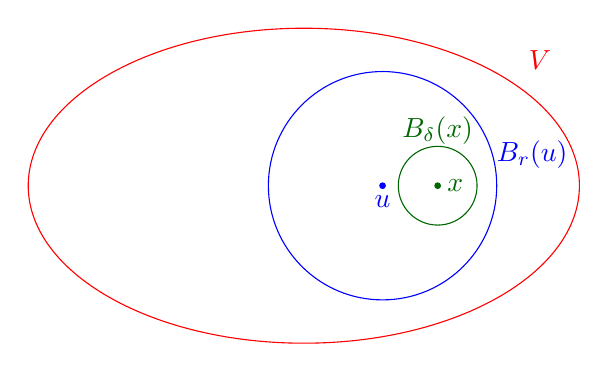
\begin{tikzpicture}
			\draw[red] (0,0) circle [x radius=3.5cm, y radius=2cm] ;
			\draw (3,1.6) node[red]{$V$};
			\draw [blue] (1,0) circle (1.45cm) ;
			\filldraw[blue] (1,0) circle (1pt) node[anchor=north]{$u$};
			\draw (2.9,0.4) node[blue]{$B_r(u)$};
			\draw [green!40!black] (1.7,0) circle (0.5cm) node [yshift=0.7cm]{$B_{\delta}(x)$} ;
			\filldraw[green!40!black] (1.7,0) circle (1pt) node[anchor=west]{$x$};
		\end{tikzpicture}
	\end{center}

	Given $x\in B_r(u)\subset V$, we want $\delta>0$ such that $x\in B_{\delta} (x)\subset B_r(u)\subset V$. Let $d=d(u,x)$. Choose $\delta $ such that $d+\delta<r$ (e.g. $\delta<\frac{r-d}{2}$)

	If $y\in B_{\delta}(x)$ we will be done by showing that $d(u,y)<r$ but $$d(u,y)\leq d(u,x)+d(x,y)<d+\delta<r$$
\end{myproof}

\cor{}{By the result of the proof, we can then show...}
\mlenma{}{Suppose $\vec{v_1}, \dots, \vec{v_n} \in \RR[n]$ is subspace of $\RR^n$.}
\mprop{}{$1 + 1 = 2$.}

\section{Random}
\dfn{Normed Linear Space and Norm $\boldsymbol{\|\cdot\|}$}{Let $V$ be a vector space over $\bbR$ (or $\bbC$). A norm on $V$ is function $\|\cdot\|\ V\to \bbR_{\geq 0}$ satisfying \begin{enumerate}[label=\bfseries\tiny\protect\circled{\small\arabic*}]
		\item \label{n:1}$\|x\|=0 \iff x=0$ $\forall$ $x\in V$
		\item \label{n:2}	$\|\lambda x\|=|\lambda|\|x\|$ $\forall$ $\lambda\in\bbR$(or $\bbC$), $x\in V$
		\item \label{n:3} $\|x+y\| \leq \|x\|+\|y\|$ $\forall$ $x,y\in V$ (Triangle Inequality/Subadditivity)
	\end{enumerate}And $V$ is called a normed linear space.

	$\bullet $ Same definition works with $V$ a vector space over $\bbC$ (again $\|\cdot\|\to\bbR_{\geq 0}$) where \ref{n:2} becomes $\|\lambda x\|=|\lambda|\|x\|$ $\forall$ $\lambda\in\bbC$, $x\in V$, where for $\lambda=a+ib$, $|\lambda|=\sqrt{a^2+b^2}$ }


\ex{$\bs{p-}$Norm}{\label{pnorm}$V={\bbR}^m$, $p\in\bbR_{\geq 0}$. Define for $x=(x_1,x_2,\cdots,x_m)\in\bbR^m$ $$\|x\|_p=\Big(|x_1|^p+|x_2|^p+\cdots+|x_m|^p\Big)^{\frac1p}$$(In school $p=2$)}
\textbf{Special Case $\bs{p=1}$}: $\|x\|_1=|x_1|+|x_2|+\cdots+|x_m|$ is clearly a norm by usual triangle inequality. \par
\textbf{Special Case $\bs{p\to\infty\ (\bbR^m$ with $\|\cdot\|_{\infty})}$}: $\|x\|_{\infty}=\max\{|x_1|,|x_2|,\cdots,|x_m|\}$\\
For $m=1$ these $p-$norms are nothing but $|x|$.
Now exercise
\qs{}{\label{exs1}Prove that triangle inequality is true if $p\geq 1$ for $p-$norms. (What goes wrong for $p<1$ ?)}
\sol{\textbf{For Property \ref{n:3} for norm-2}	\subsubsection*{\textbf{When field is $\bbR:$}} We have to show\begin{align*}
		         & \sum_i(x_i+y_i)^2\leq \left(\sqrt{\sum_ix_i^2} +\sqrt{\sum_iy_i^2}\right)^2                                       \\
		\implies & \sum_i (x_i^2+2x_iy_i+y_i^2)\leq \sum_ix_i^2+2\sqrt{\left[\sum_ix_i^2\right]\left[\sum_iy_i^2\right]}+\sum_iy_i^2 \\
		\implies & \left[\sum_ix_iy_i\right]^2\leq \left[\sum_ix_i^2\right]\left[\sum_iy_i^2\right]
	\end{align*}So in other words prove $\langle x,y\rangle^2 \leq \langle x,x\rangle\langle y,y\rangle$ where
	$$\langle x,y\rangle =\sum\limits_i x_iy_i$$

	\begin{note}
		\begin{itemize}
			\item $\|x\|^2=\langle x,x\rangle$
			\item $\langle x,y\rangle=\langle y,x\rangle$
			\item $\langle \cdot,\cdot\rangle$ is $\bbR-$linear in each slot i.e. \begin{align*}
				      \langle rx+x',y\rangle=r\langle x,y\rangle+\langle x',y\rangle	\text{ and similarly for second slot}
			      \end{align*}Here in $\langle x,y\rangle$ $x$ is in first slot and $y$ is in second slot.
		\end{itemize}
	\end{note}Now the statement is just the Cauchy-Schwartz Inequality. For proof $$\langle x,y\rangle^2\leq \langle x,x\rangle\langle y,y\rangle $$ expand everything of $\langle x-\lambda y,x-\lambda y\rangle$ which is going to give a quadratic equation in variable $\lambda $ \begin{align*}
		\langle x-\lambda y,x-\lambda y\rangle & =\langle x,x-\lambda y\rangle-\lambda\langle y,x-\lambda y\rangle                                       \\
		                                       & =\langle x ,x\rangle -\lambda\langle x,y\rangle -\lambda\langle y,x\rangle +\lambda^2\langle y,y\rangle \\
		                                       & =\langle x,x\rangle -2\lambda\langle x,y\rangle+\lambda^2\langle y,y\rangle
	\end{align*}Now unless $x=\lambda y$ we have $\langle x-\lambda y,x-\lambda y\rangle>0$ Hence the quadratic equation has no root therefore the discriminant is greater than zero.

	\subsubsection*{\textbf{When field is $\bbC:$}}Modify the definition by $$\langle x,y\rangle=\sum_i\overline{x_i}y_i$$Then we still have $\langle x,x\rangle\geq 0$}

\section{Algorithms}
\begin{algorithm}[H]
\KwIn{This is some input}
\KwOut{This is some output}
\SetAlgoLined
\SetNoFillComment
\tcc{This is a comment}
\vspace{3mm}
some code here\;
$x \leftarrow 0$\;
$y \leftarrow 0$\;
\uIf{$ x > 5$} {
    x is greater than 5 \tcp*{This is also a comment}
}
\Else {
    x is less than or equal to 5\;
}
\ForEach{y in 0..5} {
    $y \leftarrow y + 1$\;
}
\For{$y$ in $0..5$} {
    $y \leftarrow y - 1$\;
}
\While{$x > 5$} {
    $x \leftarrow x - 1$\;
}
\Return Return something here\;
\caption{what}
\end{algorithm}

\end{document}
